% TREC 2026 AutoJudge notebook paper, team IRIS-MST.
% Builds on Overleaf as is (acmart is preinstalled there). Compiler: pdfLaTeX or XeLaTeX.
% Red bracketed text marks something still to fill in. Search for \pending.
\documentclass[sigconf,nonacm]{acmart}

\settopmatter{printacmref=false, printccs=false, printfolios=true}

\usepackage{booktabs}
\usepackage{multirow}
\usepackage{pgfplots}
\pgfplotsset{compat=1.18}
\usepackage{listings}
\lstset{basicstyle=\ttfamily\scriptsize, breaklines=true, columns=fullflexible,
  frame=single, framesep=3pt, xleftmargin=4pt, xrightmargin=4pt}

\hyphenation{Nugget-Recall Cor-rob-o-rate}

% Red marker for anything not final yet.
\newcommand{\pending}[1]{\textcolor{red}{[#1]}}
\newcommand{\tauap}{\ensuremath{\tau_{\mathrm{AP,b}}}}
\newcommand{\judge}[1]{\textsf{#1}}
% System names in typewriter type, allowed to break after a hyphen.
\makeatletter\g@addto@macro{\UrlBreaks}{\do\-}\makeatother
\newcommand{\run}[1]{\nolinkurl{#1}}
\setlength{\emergencystretch}{1.5em}
% Runs the organizers executed from our code submissions.
\newcommand{\org}{$^{\dagger}$}

\begin{document}

\title{IRIS-MST at TREC 2026 AutoJudge}
\subtitle{Answer Keys from the Question and Corroboration from the Pool}

\author{Utshab Kumar Ghosh}
\affiliation{%
  \institution{Missouri University of Science and Technology}
  \city{Rolla} \state{MO} \country{USA}}
  \orcid{0000-0003-3096-6909}
  \email{u.ghosh@mst.edu}

\author{Shubham Chatterjee}
\affiliation{%
  \institution{Missouri University of Science and Technology}
  \city{Rolla} \state{MO} \country{USA}}
  \orcid{0000-0002-6729-1346}
  \email{shubham.chatterjee@mst.edu}
\renewcommand{\shortauthors}{IRIS-MST at TREC 2026 AutoJudge}

\begin{abstract}
TREC 2026 AutoJudge asks for automatic judges that rank the systems of a host
track the way human assessors would. We submitted two judges that start from
opposite assumptions. \judge{NuggetRecall} has an LLM write an answer key of 8 to
20 facts from the request alone, before it sees any response, and then checks each
response against the whole key in one call. \judge{Corroborate} uses no LLM. It
pools the sentences of all responses to a topic and counts how many distinct teams
state each claim. The scored team is left out of that count, so a team cannot vote
for its own claims. On the pilots with human truth, the two judges do best on
different measures. \judge{NuggetRecall} is our stronger judge on nugget coverage,
and in the organizers' run of our code with gpt-oss-120b it reaches 0.839 Kendall's
$\tau$ on short RAG answers. \judge{Corroborate} is our stronger judge on F1 for
long reports and fails on short answers. The judge model mattered more than any
other choice we measured. Ranking runs within each topic before averaging helped a
little on short answers and hurt a little on long reports. We also describe six
ways our judges failed, or would have failed, during development without raising
an error, and the checks that caught them.
\end{abstract}

\keywords{automatic evaluation, LLM judges, nugget evaluation, pooling, RAG}

\maketitle

\section{Introduction}

Human assessment is the slowest and most expensive part of a TREC track. Large
language models (LLMs) can grade answers for a fraction of the cost, and several
studies find that system rankings built from their grades often agree with rankings
built from human
grades~\cite{faggioli2023perspectives,thomas2024predict,upadhyay2024umbrela,pradeep2025greatnugget}.
Where such grades can stand in for human assessment, and where they break, is
still open. TREC 2026 AutoJudge turns that question into a shared
task~\cite{autojudge2026}. A participant builds a judge. The judge reads the
anonymized runs of a host track and ranks the systems that produced them. It is
scored by how closely its ranking matches the ranking that human assessors
produce.

We built two judges that start from opposite assumptions. \judge{NuggetRecall}
assumes that the request alone says what a good answer must contain. An LLM writes
an answer key of facts before it sees any response, in the tradition of nugget
evaluation~\cite{voorhees2003qa,lin2006methods,pradeep2024initial}, and then
checks each response against that key. \judge{Corroborate} uses no LLM. It
assumes that a claim many independent teams make is probably one that matters. It
pools the sentences of all responses to a topic, counts how many distinct teams
state each claim, and scores a response by the claims it shares with other teams.
The idea comes from pooling in retrieval evaluation, where the merged output of
many systems decides which documents get judged~\cite{zobel1998reliable}, and from
work that ranks systems from that pool without any human
judgments~\cite{soboroff2001ranking}.

This paper makes four contributions.
\begin{itemize}
  \item Two complete judges, each submitted as data and as code.
    \judge{Corroborate} never lets a team vote for its own claims. A claim needs
    two teams to enter the bank, and it is weighted by the number of teams other
    than the scored one that state it. This is a team-level version of the
    leave-one-run-out test of pool bias of~\citet{zobel1998reliable}.
  \item Evidence from the pilots that the two judges do best on different human
    measures. On long reports \judge{NuggetRecall} is our stronger judge on nugget
    coverage and \judge{Corroborate} on F1. On short answers \judge{Corroborate}
    trails on both truth measures.
  \item Measurements of what matters inside an LLM judge. The judge model mattered
    most. Ranking runs within each topic before averaging gave a small gain on
    short answers and a small loss on long reports.
  \item Six ways our judges failed, or would have failed, during development
    without raising an error. Several produced a leaderboard that looked plausible.
    We describe the checks that caught them.
\end{itemize}

Every pilot score in this paper comes from the organizers' evaluation on TIRA,
and every comparison with other entries is informal. Test-set results will be
added once the organizers release them.

\section{Task, Data and Evaluation}
\label{sec:task}

\subsection{The task}

Each AutoJudge dataset holds the topics of a host track and the anonymized runs
submitted to it. A run contains one response per topic. A response is a list of
sentences, each with optional citations to documents. It also carries metadata that
names the run and an anonymized team. A judge reads all of this and writes a
leaderboard with one score per run, topic and measure, plus an aggregate row for
each run. A judge may emit several measures.

A complete submission has two parts. The \emph{data submission} is the set of
leaderboards the judge produces on the test sets. The \emph{code submission} is the
judge itself, packaged as a container that TIRA runs. This lets the organizers rerun
it with an LLM of their choice. An LLM judge must also reproduce its own
leaderboard with the LLM endpoint (the server that answers its calls) switched
off. It does so by replaying every call from its prompt cache, a stored record of
each prompt and the reply it received.

\subsection{Data}

Table~\ref{tab:data} lists the datasets. One test set comes from the TREC 2026
RAG (retrieval-augmented generation) track, whose responses are short cited
answers. The other comes from the TREC 2026 RAGTIME track, whose responses are
long cited reports. Teams often submit several close variants of one pipeline,
so the table counts teams as well as runs. Both test releases are in English.
They carry the text of cited documents inline, for 99.1\% and 99.7\% of
responses.

The three pilot datasets come from TREC 2025 and have human assessments. No release
ships them, though. The truth stays on the TIRA server. The only way to measure a
judge is to run it on a pilot, upload the leaderboard and read back the correlation
the organizers compute. Every pilot number in this paper was measured this way.
Of the pilots, rag25-gen is closest to rag26 and ragtime25 is closest to ragtime26.
Each topic in dragun-repgen is a news article. The report should help a reader
assess it. DRAGUN topics do not fit the AutoJudge request format, so the organizers
converted them. Next to the original article topics, the release ships a converted
file. That is the file its own configuration names. In the converted file each
topic has a question as title, a summary of the article's claims (about 1.4\,KB) as
problem statement and a fact-checker background. The copy on TIRA instead gives
the judge only the article's headline (Section~\ref{sec:dragun}).

\begin{table}
  \caption{Datasets. The test sets have no released truth. The pilots have human
  truth, held on TIRA.}
  \label{tab:data}
  \small
  \setlength{\tabcolsep}{3pt}
  \begin{tabular}{@{}llrrrr@{}}
    \toprule
    Dataset & Kind & Runs & Teams & Topics & Responses\\
    \midrule
    rag26 (test)          & short answers & 83 & 25 & 119 & 9,877\\
    ragtime26 (test)      & long reports  & 49 & 10 & 103 & 5,047\\
    \midrule
    rag25-gen (pilot)     & short answers & 51 & 18 & 105 & 5,332\\
    ragtime25 (pilot)     & long reports  & 59 & 13 & 122 & 7,198\\
    dragun-repgen (pilot) & news reports  & 28 & 9  & 30  & 840\\
    \bottomrule
  \end{tabular}
\end{table}

\subsection{How judges are scored}
\label{sec:scoring}

TIRA correlates each measure a judge emits with each human truth measure, over the
systems' aggregate scores. It uses two rank correlations. Kendall's
$\tau$~\cite{kendall1938new} measures how often two rankings put a pair of
systems in the same order. \tauap\ is the AP rank correlation~\cite{yilmaz2008new} in its
tie-aware form~\cite{urbano2017ties}. It gives more weight to agreement at the top
of the ranking. For each truth measure TIRA reports the maximum over
the judge's measures.

On 2026-10-09 the organizers re-scored every entry on rag25-gen and ragtime25
against a revised set of truth measures. For rag25-gen there are now two, Strict
Vital Score and Sub Coverage. For ragtime25 there are Nugget Coverage Macro and F1 Macro, shortened below to Nugget Coverage and F1. We leave out its third measure, Citation Support, which currently reads
0.000 for every entry. On dragun-repgen TIRA still reports a single maximum over
all its truth measures. The organizers have not described the revised measures in
detail. Where we read meaning into them below, we go by their names. We made our
design choices under the earlier scoring, which reported one maximum over all truth
measures on every pilot. This paper gives the current numbers and notes where the
two scorings disagree.

Three features of the scoring shaped both judges. First, only the best measure
counts, so emitting several well-motivated measures costs nothing. Each judge
therefore emits four or five. The same rule flatters a system with many
measures, because the best one is picked after the fact. Two of our rows in Table~\ref{tab:pilots} emit a single measure and so get no such help. These are ``rank only'' and the ensemble (Section~\ref{sec:results}).
Second, the earlier scoring also reported the minimum over all pairs of measures.
We therefore oriented every measure so that higher is better. Third, the
organizers' evaluator breaks ties in a judge's scores by input order. A coarse
score, one with few distinct values, therefore loses agreement at random. That is
why all our measures are continuous.

\subsection{Data policy}

The track limits what developers may look at, because the test responses are
themselves the test set. Section~\ref{sec:disclosure} explains how we kept to these limits. It also describes the one engineering change that followed a failure count on the test data.

\section{NuggetRecall}
\label{sec:nuggetrecall}

\judge{NuggetRecall} makes two kinds of LLM call. One call per topic writes an
answer key. One call per response then checks that response against the whole key.
The number of calls therefore grows with topics plus responses, not with responses
times facts. All of rag26 takes 9,838 judging calls. Its 39 responses with no text
score zero without a call.

\subsection{An answer key from the request alone}

For each topic, the LLM receives the request, which is the topic's title, problem
statement and background in a fixed order. We ask it for 8 to 20
self-contained facts that a complete, high-quality response should contain, with
the most important first. Each fact carries a tag. VITAL means a response that
leaves the fact out is clearly incomplete. OKAY means the fact is useful
supporting detail. Figure~\ref{fig:key} shows part of one key.
Appendix~\ref{app:prompts} gives both prompts in full.

The model never sees a response at this step. The AutoJudge framework enforces
this. Our workflow declares that the key does not depend on responses, so none are
passed in. Keeping responses out has three effects. A verbose system cannot shape
the key. The key can hold a fact that every system missed, which a key mined from
the responses cannot. And because the key comes from the topic alone, the data
policy lets us read it for any topic.

The parser accepts numbered lines that carry a VITAL or OKAY tag. It drops
duplicates and stops at 20 facts. A model that ignores the requested range
therefore cannot inflate the recall denominator. If a reply has fewer than two
usable facts, we retry with a fixed suffix appended to the prompt. If every attempt
fails, the topic falls back to a title-only key, a single fact made from its title. That never
happened with Qwen3-30B, our main judge model (Section~\ref{sec:setup}), on any pilot or test set. With gpt-oss-20b it happened on 5
of 122 ragtime25 topics and on 3 of 103 ragtime26 topics.

\begin{figure}
  \small
  \fbox{\parbox{0.94\columnwidth}{%
    \textbf{Request} (rag25-gen, topic 464, shortened). I want a thorough
    understanding of what makes up a community, including its definitions in
    various contexts like science [\ldots] I'm also interested in related terms
    like grassroots organizations, how communities set boundaries and
    priorities, and their roles in important areas such as preparedness and
    nation-building.

    \smallskip
    \textbf{Answer key} (5 of 20 facts).\\[2pt]
    \textsc{vital}\quad In ecology, a community refers to all the interacting
    populations of different species living in a particular area and sharing
    resources.\\[2pt]
    \textsc{vital}\quad Grassroots organizations are community-driven groups
    formed by local individuals to address specific social, environmental, or
    political issues from the bottom up [\ldots]\\[2pt]
    \textsc{vital}\quad Communities establish boundaries through shared identity,
    cultural norms, geographic limits, or formal rules, which help define
    membership and exclusion.\\[2pt]
    \textsc{okay}\quad Community boundaries can be fluid and change over time due
    to migration, cultural shifts, or political reorganization.\\[2pt]
    \textsc{okay}\quad Preparedness efforts in communities often involve
    collaboration with government agencies, NGOs, and emergency services.}}
  \caption{Part of an answer key that Qwen3-30B wrote from the request alone. The
  full key has 8 VITAL and 12 OKAY facts. The topic is the first one in the
  rag25-gen topics file. We did not pick it by hand.}
  \label{fig:key}
\end{figure}

\subsection{Checking each response in one call}

A single call judges each response against the whole key. The prompt holds the
request, the response and the numbered facts. The response appears as its
sentences joined with spaces. It is capped at 40,000 characters, a length no pilot
response reached. Citations and cited documents are left out, so
\judge{NuggetRecall} does not judge attribution (whether the cited documents back
what the response says). The prompt asks for one label per fact. The label is
\emph{support} if the response clearly states the fact. It is \emph{partial} if the
response states part of it or hedges it. Anything else gets \emph{no}. The model is
told to judge meaning rather than wording and to use no outside knowledge. The
sampling temperature is 0.

A reply is rejected unless it labels at least 80\% of the facts, rounded down to a
whole number. We do not accept a shorter reply and fill its gaps with \emph{no}.
That would invent misses and quietly understate the system. In an accepted reply,
the few facts left unlabeled count as \emph{no}. A rejected reply is retried up to
twice with a fixed suffix. The suffix changes the prompt and with it the cache key,
the lookup key for a stored reply. Since the suffix is fixed, replay stays
deterministic. A response that is still unreadable after three attempts scores
zero. We log how many there are. A reasoning model writes out intermediate steps
before its final answer. So its reply may hold a visible reasoning block before
the labels. The parser strips that block.

\subsection{Measures}

Let $K_q$ be the facts in the key for topic $q$ and $V_q \subseteq K_q$ the vital
ones. Let $\ell_{r,k}$ be the label that response $r$ received for fact $k$.
Lenient credit is $c(\text{support})=1$, $c(\text{partial})=0.5$ and
$c(\text{no})=0$. Strict credit $c'$ gives 1 to support only. Then
\begin{align}
  \texttt{NR\_VITAL}(r,q) &= \frac{1}{|V_q|}\sum_{k\in V_q} c(\ell_{r,k}),\\
  \texttt{NR\_WEIGHTED}(r,q) &= \frac{\sum_{k\in K_q} w_k\, c(\ell_{r,k})}{\sum_{k\in K_q} w_k},
\end{align}
with $w_k=1$ for vital facts and $0.5$ for okay ones. \texttt{NR\_ALL} is
\texttt{NR\_VITAL} taken over all of $K_q$. \texttt{NR\_VITAL\_STRICT} is
\texttt{NR\_VITAL} with $c'$. If a key has no vital fact, vital recall falls back to
recall over all facts. A system's score is its mean over topics. A missing response
counts as zero.

The fifth measure, \texttt{NR\_RANK}, uses the same judgments but aggregates them
differently. On each topic, every run gets the share of the other runs it beats on
\texttt{NR\_VITAL}, with ties split evenly. This within-topic percentile is
\begin{equation}
  \label{eq:percentile}
  p_q(r) = \frac{|\{r' : s_q(r') < s_q(r)\}| + \tfrac{1}{2}\,|\{r'\neq r : s_q(r') = s_q(r)\}|}{R_q - 1},
\end{equation}
where $s_q$ is the score on topic $q$ and $R_q$ is the number of runs with a
response on that topic. \texttt{NR\_RANK} is the mean of $p_q(r)$ over topics. A
plain mean over topics lets an easy topic, where every system scores high, count as
much as one that separates systems. Ranking within each topic before averaging
removes that difficulty effect. This follows the spirit of score
standardization~\cite{webber2008standardization}, which turns each topic's scores
into $z$-scores using their mean and standard deviation. We use a percentile and
not a $z$-score because the framework fills a missing cell with 0. Zero is the
right floor for a percentile but the wrong one for a $z$-score.

\subsection{Room to think for reasoning models}
\label{sec:budget}

The organizers run submitted code with gpt-oss models, which reason before they
answer. Each call has a reply budget, the most tokens the model may generate. A
reasoning model that uses up its budget stops in mid-thought and never writes its
labels. Retrying with the same budget cannot help. So each retry doubles the
budget, from 4,096 tokens to 8,192 and then 16,384. That still fits a context of
32,768 tokens. The first attempt keeps its original budget, so existing cache
entries still match. Section~\ref{sec:failures} shows the effect.

\subsection{Caching and replay}

All calls go through the organizers' minima-llm client~\cite{minimallm}. Its SQLite
cache builds each key from the model, the messages, the temperature and the reply
budget. The endpoint is not part of the key. Responses are sorted by run id before
any prompt is built, so prompts are byte-identical from one execution of the judge
to the next. That is what lets TIRA replay the judge from its cache with the
endpoint switched off.

\section{Corroborate}
\label{sec:corroborate}

\judge{Corroborate} builds its reference from the one resource every dataset has,
the responses themselves. It needs no LLM, no document collection and no network
access.

\subsection{Pooling sentences into claims}

For each topic we take every sentence of every response and normalize it. We drop
fixed boilerplate and any sentence shorter than five words. Each sentence is
embedded with bge-base-en-v1.5~\cite{xiao2023cpack}, a model that maps sentences
with similar meaning to nearby vectors. We then cluster them greedily, in a fixed
order by run id and sentence position. A sentence joins the cluster whose first
sentence, the leader, is most similar to it, as long as the cosine similarity is at
least $\theta=0.80$. Otherwise it starts a new cluster. The fixed order makes the
result independent of file order. Each cluster records the set of teams $T(c)$
whose responses contributed to it.

Clustering also does the matching. A response covers a cluster when one of its own
sentences ended up in it, so we need no separate retrieval step.

Both $\theta$ and the partial-credit cutoff of 0.62 used below come from similarities on a small synthetic dataset. It ships with the task's starter kit, the template code participants build their judges from. There a true paraphrase scored about 0.83
while an unrelated sentence on the same topic got about 0.61. Neither was swept on
the pilots.

\subsection{The claim bank}

A cluster enters the topic's bank only if at least two teams contributed to it. It
must also be specific to the topic. Specificity is the cosine similarity between
the cluster's leader and the topic text, with a floor of 0.50. The bank keeps at
most the 40 clusters with the most teams. Votes are counted per team, never per
run. Otherwise a team that submits five variants of one pipeline would
vote five times for its own phrasing. We set the cap of 40 and the five-word
minimum by hand and did not tune them.

\subsection{Leave-one-team-out weighting}

A response's own sentences are part of the pool behind its bank. Two
rules keep a team from voting for its own claims. First, a cluster needs at least
two teams to enter the bank. So a claim made by only one team is never scored.
Second, when we score a response from team $t$, each cluster gets the weight
\begin{equation}
  w_t(c) = |T(c) \setminus \{t\}|,
\end{equation}
the number of other teams that state it. Without this weight, a team's own
sentences would raise the weight of the claims it is scored on. Every bank
cluster has at least two teams, so the weight is never below one. Leaving the
scored team out of every weight is what we mean by leave-one-team-out.

The scheme is a team-level version of the leave-one-run-out test
of~\citet{zobel1998reliable}. That test removes from the pool whatever one run
alone contributed. Zobel used it to measure pool bias. We use the same idea to
correct for it.

\subsection{Measures}

Coverage is soft and allows partial credit. For a bank cluster $c$, response $r$
gets $\mathrm{cov}_r(c)=1$ if one of its sentences was assigned to $c$. The same
holds if its most similar sentence reaches $\theta$. Below 0.62 the credit is 0. In
between, when the best similarity falls in $[0.62, \theta)$, the credit is the
entailment probability from a cross-encoder. A cross-encoder reads both texts
together and scores the pair directly, instead of comparing separate embeddings.
Ours is nli-deberta-v3-base, a DeBERTaV3 model~\cite{he2023debertav3} fine-tuned
for natural language inference. That is the task of deciding whether one text
entails, contradicts or is neutral to another. Coverage is then
\begin{equation}
  \texttt{NCOV}(r) = \frac{\sum_{c} w_t(c)\,\mathrm{cov}_r(c)}{\sum_{c} w_t(c)}.
\end{equation}

\texttt{NPREC} is the share of the response's own sentences that sit in a
topic-specific cluster also stated by at least one other team. Because it is
normalized by length, padding and claims nobody else makes pull it down.
\texttt{NF1} is the harmonic mean of \texttt{NCOV} and \texttt{NPREC}.
\texttt{NF1\_RANK} is the within-topic percentile of \texttt{NF1}, as in
Equation~\ref{eq:percentile}. 

\texttt{CITE} measures citation support. For each cited sentence we check the first
three documents it cites. We split each document into chunks of at most 1,200
characters and use only its first six. For each document we take the chunk closest
to the sentence by embedding similarity. The cross-encoder's probability that this
chunk entails the sentence is the document's support. A sentence's support is the
highest over its documents. \texttt{CITE} averages it over the cited sentences that
have at least one document present. The path is chosen per dataset. When fewer
than half the responses carry document text, \texttt{CITE} uses citation overlap
instead. This is the mean share of other teams citing the same documents, times the
share of sentences that cite anything. Both test sets carry the text, so on them
\texttt{CITE} uses entailment.

\subsection{Why a pooled bank is not circular}

Two arguments support the design. First, the human reference is itself built from
a pool. In TREC RAG, the documents that systems retrieved are pooled and nugget
banks are drafted from them. Assessors then vet the
banks~\cite{pradeep2024initial}. That pool holds documents rather than answers, so
the analogy is loose. Still, in both cases the reference comes from what the
systems produced. Second, a fact that no system states cannot enter the bank. It
would give every system the same zero anyway, so it cannot change their order.

The real risk is that consensus pulls every system toward the median. That would
hurt most at the top of the ranking, where \tauap\ weighs errors most.
Section~\ref{sec:analysis} suggests this is what happens on short answers. We have
not tested it directly.

\subsection{Cost}

Our first version issued one matrix-vector product per sentence. Nearly all of its
time went to starting and joining thread pools. We now cluster in blocks of 512
sentences, which cut pooling from 13.0 to 1.04 seconds per topic. A test checks
that the output is identical to the sequential version. On one GPU, a full run
takes 73 minutes on rag26 and 22 minutes on ragtime26. On CPU alone, a pilot took
about eight hours.

\section{Experimental Setup}
\label{sec:setup}

\paragraph{LLMs.} Our data submissions use two judge models. The first is
Qwen3-30B-A3B-Instruct-2507 from the Qwen3 family~\cite{yang2025qwen3}, with its
weights in FP8, a low-precision floating-point format. We call it Qwen3-30B. It is a mixture-of-experts
model. Each token passes through only a few expert sub-networks, so about 3B
parameters are active per token. This 2507 Instruct release has no thinking mode,
so it writes no reasoning block. The second, gpt-oss-20b~\cite{openai2025gptoss},
is a reasoning model. We also ran Qwen2.5-7B-Instruct~\cite{qwen2025qwen25} on one
pilot, because the organizers named it among the models they would use. We served
all three with vLLM 0.13.0~\cite{kwon2023vllm}, an open-source LLM serving engine,
on one NVIDIA RTX 6000 Ada GPU with 48\,GB of memory. We allowed a context of
32,768 tokens and up to 64 concurrent sequences. A full run with Qwen3-30B
took 30 minutes on rag26 and 14 minutes on ragtime26. gpt-oss-20b is slower. It
took 99 minutes on ragtime25, at about 40 seconds per call.

\paragraph{Reply budgets.} Our main data submission is \run{nuggetrecall-best} (Table~\ref{tab:submissions}). In it and on the pilots, our Qwen3-30B and Qwen2.5-7B runs capped replies at
1,536 tokens for the key and 1,024 for judging. We later raised both to 4,096 for
reasoning models. Neither Qwen model reasons before it answers. vLLM also recorded
no Qwen3-30B reply that reached the old limit. Our gpt-oss-20b runs used 4,096
tokens on every attempt, except the rag26 run, which had the growing budget of
Section~\ref{sec:budget}.

\paragraph{Runs by the organizers.} The organizers ran our code submissions on
TIRA with models they chose. We made two \judge{NuggetRecall} code submissions, \run{rank-dioptre} and \run{grave-node} (Section~\ref{sec:submissions}). On the pilots the organizers ran \run{rank-dioptre}, which keeps
4,096 tokens on every attempt. On rag25-gen they paired it with gpt-oss-120b. On
dragun-repgen they ran it with Qwen2.5-7B-Instruct, gpt-oss-20b and gpt-oss-120b.
Our \judge{Corroborate} submission, \run{lead-racer}, ran on CPU on all three
pilots. On the test sets they ran \run{lead-racer}, plus \run{rank-dioptre} and
\run{grave-node} with the same three models. \run{grave-node} also got a fourth
model, listed on TIRA as Qwen3.8-27B-FP8. Tables mark organizer runs with \org.

\paragraph{Encoders.} \judge{Corroborate} uses bge-base-en-v1.5 to embed
sentences and the nli-deberta-v3-base cross-encoder to check entailment. Both run
on a GPU when one has at least 6\,GB free, or else on CPU with eight threads.

\paragraph{Validation.} We fitted nothing on the test sets. Every choice we made by
score came from the pilots. Three \judge{Corroborate} constants have other
sources. The similarity threshold $\theta$ and the partial-credit cutoff come from the synthetic
dataset (Section~\ref{sec:corroborate}). The specificity floor is based on the
encoder's range (Section~\ref{sec:floor}). One engineering change followed an
observation on test data. On the first pass, 27\% of the rag26 judgments by gpt-oss-20b came back
unreadable. So we added the growing reply budget of Section~\ref{sec:budget} and
asked the organizers to treat the code submission carrying it as our main one. We
saw only that count and vLLM's count of replies cut off at the length limit. We
never saw a response, a grade or any truth data.

\judge{NuggetRecall} is not deterministic across runs (Section~\ref{sec:noise}).
\judge{Corroborate} is. Its output on our GPU matched the organizers' CPU run to
within 0.002. Section~\ref{sec:noise} measures how much \judge{NuggetRecall} varies from run to run.

\paragraph{Code submission.} Our machines have no container runtime such as
Docker, so we build and submit the containers from GitHub Actions. Before each
submission the workflow runs the test suite. Next it fills the prompt
cache by running the judge once against a stub LLM endpoint, a stand-in for a
real model. Then it runs the container with the endpoint switched off. To pass, the container must
reproduce its own leaderboard from that cache. That leaderboard must also actually
rank systems apart. The starter base image ships Python 3.11.0rc1, a release
candidate. On it, a current transformers and PyTorch stack fails at import, so our
image installs its own Python 3.12.

\section{Results on the Pilots}
\label{sec:results}

Table~\ref{tab:pilots} shows the current TIRA scores on rag25-gen and ragtime25.
Table~\ref{tab:dragun} shows them on dragun-repgen. The field median and field best
are taken over every entry on each leaderboard, as read on 2026-10-19. That covers
385 entries on rag25-gen, 206 on ragtime25 and 139 on dragun-repgen. Many entries
are variants from the same team, so a rank among entries is only a rough guide. The
length row is the organizers' baseline judge. It scores each response by how long
it is.

\begin{table*}
  \caption{Pilot results, read from TIRA on 2026-10-19. Each cell is the
  correlation with one human truth measure, taking the maximum over the judge's
  measures. K is Kendall's $\tau$. \org\ marks runs the organizers made from our
  code submissions. These are \run{rank-dioptre} for \judge{NuggetRecall} and
  \run{lead-racer} for \judge{Corroborate}. Bold marks our best in each column.
  n/a means not run.}
  \label{tab:pilots}
  \small
  \begin{tabular}{@{}ll cc cc c cc cc@{}}
    \toprule
    & & \multicolumn{4}{c}{rag25-gen (short answers)} & & \multicolumn{4}{c}{ragtime25 (long reports)}\\
    \cmidrule{3-6}\cmidrule{8-11}
    & & \multicolumn{2}{c}{Strict Vital Score} & \multicolumn{2}{c}{Sub Coverage} & & \multicolumn{2}{c}{Nugget Coverage} & \multicolumn{2}{c}{F1}\\
    Judge & Model & K & \tauap & K & \tauap & & K & \tauap & K & \tauap\\
    \midrule
    Length baseline & & 0.152 & 0.119 & 0.094 & 0.063 & & 0.193 & $-$0.013 & 0.155 & $-$0.008\\
    Field median    & & 0.804 & 0.626 & 0.772 & 0.605 & & 0.726 & 0.550 & 0.583 & 0.364\\
    Field best      & & 0.906 & 0.799 & 0.866 & 0.786 & & 0.825 & 0.697 & 0.808 & 0.678\\
    \midrule
    \judge{NuggetRecall} & Qwen3-30B                & 0.783 & 0.621 & 0.788 & 0.615 & & 0.697 & 0.492 & 0.500 & 0.296\\
    \quad rank only      & Qwen3-30B                & 0.792 & 0.634 & \textbf{0.809} & \textbf{0.628} & & 0.681 & 0.475 & 0.465 & 0.243\\
    \judge{NuggetRecall} & gpt-oss-20b              & 0.783 & 0.601 & 0.736 & 0.622 & & \textbf{0.728} & \textbf{0.528} & 0.517 & 0.288\\
    \judge{NuggetRecall} & Qwen2.5-7B               & 0.604 & 0.402 & 0.654 & 0.479 & & n/a & n/a & n/a & n/a\\
    \judge{NuggetRecall} & gpt-oss-120b\org         & \textbf{0.839} & \textbf{0.710} & 0.776 & 0.616 & & n/a & n/a & n/a & n/a\\
    Ensemble             & Qwen3-30B + gpt-oss-20b  & 0.812 & 0.695 & 0.761 & 0.562 & & 0.709 & 0.486 & 0.493 & 0.257\\
    \midrule
    \judge{Corroborate}, floor 0.15 & none          & 0.257 & 0.240 & 0.323 & 0.278 & & 0.598 & 0.447 & \textbf{0.662} & \textbf{0.524}\\
    \judge{Corroborate}, floor 0.50 & none          & 0.257 & 0.240 & 0.323 & 0.278 & & 0.585 & 0.437 & 0.653 & 0.520\\
    \judge{Corroborate}, floor 0.50 & none\org      & 0.256 & 0.240 & 0.321 & 0.276 & & 0.582 & 0.437 & 0.644 & 0.511\\
    \bottomrule
  \end{tabular}
\end{table*}

\begin{table}
  \caption{Results on dragun-repgen. Each cell is the maximum over all truth
  measures and all of the judge's measures. In the Topics column, \emph{rel.} is
  the topics file named in the local release and \emph{head.} is the article
  headline alone. The headline is all that TIRA gives the judge. \org\ marks the
  organizers' runs of our code, \run{rank-dioptre} and \run{lead-racer}. $^{*}$
  marks the run made with our September code. The field rows were read on
  2026-10-19 and our later runs on 2026-10-21.}
  \label{tab:dragun}
  \small
  \setlength{\tabcolsep}{4pt}
  \begin{tabular}{@{}llccc@{}}
    \toprule
    Judge & Model & Topics & K & \tauap\\
    \midrule
    Length baseline & & & 0.391 & 0.184\\
    Field median    & & & 0.668 & 0.533\\
    Field best      & & & 0.821 & 0.700\\
    \midrule
    \judge{NuggetRecall} & Qwen3-30B$^{*}$  & rel.  & 0.141 & 0.306\\
    \judge{NuggetRecall} & Qwen3-30B        & rel.  & 0.041 & 0.173\\
    \judge{NuggetRecall} & Qwen3-30B        & head. & 0.054 & 0.239\\
    \judge{NuggetRecall} & Qwen2.5-7B       & rel.  & 0.215 & 0.312\\
    \judge{NuggetRecall} & Qwen2.5-7B       & head. & 0.190 & 0.263\\
    \judge{NuggetRecall} & Qwen2.5-7B\org   & head. & 0.587 & 0.453\\
    \judge{NuggetRecall} & gpt-oss-20b\org  & head. & 0.589 & 0.446\\
    \judge{NuggetRecall} & gpt-oss-120b\org & head. & \textbf{0.804} & \textbf{0.649}\\
    \midrule
    \judge{Corroborate}, floor 0.15 & none        & rel.  & 0.755 & 0.608\\
    \judge{Corroborate}, floor 0.50 & none        & rel.  & 0.739 & 0.516\\
    \judge{Corroborate}, floor 0.50 & none\org    & head. & 0.734 & 0.505\\
    \bottomrule
  \end{tabular}
\end{table}

The ``rank only'' row takes the exact judgments behind the Qwen3-30B row and
aggregates them with \texttt{NR\_RANK} alone (Equation~\ref{eq:percentile}). Our test-set system
\run{nuggetrecall-rank} emits the measures of both rows from the same judgments. On the pilots, its equivalent is
therefore the better of the two rows in each column. The TIRA pilot entries named
\run{nuggetrecall-rank} are separate re-runs. Section~\ref{sec:noise} uses them to
measure noise. The ensemble row emits one fused measure
(Section~\ref{sec:ensemble}). Section~\ref{sec:floor} discusses the two
\judge{Corroborate} floors.

On short answers, \judge{NuggetRecall} sits near the field median. With
gpt-oss-120b it reaches 0.839 Kendall and 0.710 \tauap\ on Strict Vital Score.
That \tauap\ ranks 20th of 385 entries. \judge{Corroborate} stays between 0.26 and
0.32 there. On long reports, which of our two judges does better depends on the
truth measure. \judge{NuggetRecall} is our best on Nugget Coverage.
\judge{Corroborate} is our best on F1, where its \tauap\ ranks 32nd of 206 entries
(Section~\ref{sec:analysis}). On dragun-repgen, \judge{Corroborate} is 8th of 139
entries on Kendall. One \judge{NuggetRecall} run with gpt-oss-120b comes 4th. But
Section~\ref{sec:dragun} shows that \judge{NuggetRecall} scores on this pilot swing
too widely to rank models.

\section{Analysis}
\label{sec:analysis}

\subsection{The two judges do best on different truth measures}

On short answers \judge{NuggetRecall} is far ahead. On rag25-gen it reaches about
0.79 Kendall on both truth measures, while \judge{Corroborate} stays at 0.26 to
0.32. One reading is that good short answers stand out by stating precise facts
that most teams did not, and a consensus bank cannot reward such facts by
construction. This fits the regression to the median we worried about when
designing \judge{Corroborate}, though other causes, such as the few sentences in a
short answer, could explain it too.

On long reports the picture splits by truth measure. On ragtime25 Nugget Coverage,
\judge{NuggetRecall} reaches 0.697 with Qwen3-30B and 0.728 with gpt-oss-20b, close
to the median of 0.726, and \judge{Corroborate} only 0.598. On F1 the order flips.
\judge{Corroborate} reaches 0.662 Kendall and 0.524 \tauap, against medians of
0.583 and 0.364, while \judge{NuggetRecall} reaches 0.47 to 0.52. If F1 has a
precision side, as its name suggests, it penalizes padding, which a recall measure
does not. \texttt{NPREC} does too, since every sentence that no other team
corroborates lowers it. TIRA reports only the maximum over our measures, so we
cannot confirm which \judge{Corroborate} measure produced its F1 score.

The two judges also rank systems differently. On our first pilot runs, Kendall
between the \texttt{NCOV} of \judge{Corroborate} and the \texttt{NR\_VITAL} of
\judge{NuggetRecall} is 0.51 on ragtime25 and 0.25 on rag25-gen. Between
\texttt{NPREC} and \texttt{NR\_VITAL} it is only 0.20 and $-$0.05. The four
mean-based measures of \judge{NuggetRecall} agree with one another at 0.87 to 0.97
on both pilots.

Since TIRA keeps the best of a judge's measures, one leaderboard carrying the
measures of both judges would have matched the better judge on every truth measure.
That gain would come from the scoring rule rather than from better judging, and we
submitted the judges as separate systems.

\subsection{The judge model matters most}

With the prompts held fixed, changing the LLM moved the score more than anything
else we tried. These runs also differ in code version, reply budget and server
(Section~\ref{sec:setup}), so the comparison is not fully controlled. On rag25-gen
Strict Vital Score, Qwen2.5-7B reaches 0.604, Qwen3-30B and gpt-oss-20b both reach
0.783, and gpt-oss-120b reaches 0.839 in the organizers' run of our code. We leave
dragun-repgen out of this comparison for the reasons in
Section~\ref{sec:dragun}.

The 7B model does not fail on format. Over 5,302 calls it returned no unreadable
reply. It judges less accurately. On the small synthetic dataset that ships with
the starter kit, it gave the worst run 38\% recall where Qwen3-30B gave that run
0\%, which suggests it grants partial credit too freely. We did not count its
labels by type on the pilots.

The reasoning model helps more on long reports. On ragtime25 Nugget Coverage,
gpt-oss-20b beats Qwen3-30B by 0.031 Kendall and 0.036 \tauap, although 2.9\% of
its judgments stayed unreadable and 5 of 122 topics fell back to a title-only key.
Checking twenty facts against a long report seems to reward a model that reasons
first. On F1 the two are within noise (0.517 against 0.500). On short answers they
tie on Strict Vital Score Kendall at 0.783, though gpt-oss-20b is lower on its
\tauap\ (0.601 against 0.621). On Sub Coverage gpt-oss-20b is behind on Kendall
(0.736 against 0.788) and slightly ahead on \tauap\ (0.622 against 0.615).

\subsection{DRAGUN cannot rank LLM judge settings}
\label{sec:dragun}

Our first \judge{NuggetRecall} run on dragun-repgen, with Qwen3-30B, scored 0.141.
The organizers' runs of our code scored about 0.59 with Qwen2.5-7B and with
gpt-oss-20b, and 0.804 with gpt-oss-120b. We made six more runs to find out why
(Table~\ref{tab:dragun}).

The code is not the cause. The current code with Qwen3-30B scored 0.041.

The input differs, though. The topics file named in the local release gives the
judge a question, a summary of the article's claims and a fact-checker background.
The answer keys from the organizers' runs show that the copy on TIRA gives only the
article's headline: their title field holds the headline on all 30 topics. We
rebuilt headline-only topics locally, and the two copies then behaved alike. Our
Qwen2.5-7B run on headlines agrees with the organizers' Qwen2.5-7B run at 0.73
Kendall on \texttt{NR\_VITAL}, against 0.28 for our run on the released topics. Our
\judge{Corroborate} run on headlines at floor 0.50 reproduces the organizers'
\run{lead-racer} leaderboard exactly, with Kendall 1.000 on every measure.

Matching the input did not close the gap. On headlines, our Qwen2.5-7B run scored
0.190, where the organizers' run of the same setup scored 0.587, and Qwen3-30B
scored 0.054. Two runs of the same setup can differ this much because every run
writes new answer keys, only 2 of 30 of which came out identical to the organizers'
here, and because the pilot has only 28 systems. On the 12 runs the release marks
as priority, our Qwen2.5-7B ranking and the organizers' agree at only 0.36 to 0.79
Kendall, depending on the measure.

So dragun-repgen cannot tell us which model or setting suits \judge{NuggetRecall}.
Its scores for this judge range from 0.04 to 0.80 across our runs and the
organizers' runs, and the 0.804 of gpt-oss-120b is a single run.
\judge{Corroborate} is deterministic, so its scores there are stable from run to
run. One lesson carries over to any track: check that the data you validate on
locally is what the evaluation platform feeds your judge. On rag25-gen the two
copies differ only in which field holds the request, which our judges happen to
handle. On dragun-repgen they differ in substance, and we found out only after the
deadline. TIRA does not let participants download runs on the test sets, so we
could not make the same check there.

\subsection{Ranking within each topic}

Re-aggregating the identical Qwen3-30B judgments by within-topic rank raises
rag25-gen Kendall from 0.783 to 0.792 on Strict Vital Score and from 0.788 to 0.809
on Sub Coverage, and \tauap\ by 0.013 on both. It costs no extra LLM calls, and
since the judgments are identical, the run-to-run noise of
Section~\ref{sec:noise} does not apply to this comparison. On ragtime25 it does
worse: 0.681 against 0.697 on Nugget Coverage and 0.465 against 0.500 on F1. One
possible reason is that a rank keeps only the order of runs on a topic, and on long
reports the size of the gaps between runs carries information. Because the reported
score is a maximum, emitting both forms costs nothing, which is what our
\run{nuggetrecall-rank} systems do.

\subsection{Averaging two LLMs helps at the top, on one truth measure}
\label{sec:ensemble}

Our ensemble ranks runs within each topic by the \texttt{NR\_VITAL} of each model
and averages the two percentiles with equal weight. No weight was fitted. On
rag25-gen Strict Vital Score its \tauap\ is 0.695, 34th of 385 entries, against
0.634 for Qwen3-30B (the better of its two rows) and 0.601 for gpt-oss-20b alone. Two judges that make different
mistakes seem to cancel some of each other's errors about the best systems. On Sub
Coverage, though, the ensemble is worse than either model on \tauap, at 0.562
against 0.628 and 0.622. On ragtime25 it never beats gpt-oss-20b alone, since
averaging dilutes the stronger judge.

We chose the ensemble for rag26 under the earlier scoring, which reported one
maximum over both rag25-gen truth measures and so showed only the gain. Under the
current scoring the gain holds for one truth measure and reverses for the other. Our
other rag26 systems hedge that choice.

\subsection{Length is a weak shortcut under the current truth}

The organizers' length baseline reaches 0.152 Kendall on rag25-gen and 0.193 on
ragtime25 under the current truth measures. Under the earlier scoring it reached
0.558 on ragtime25, and we spent design effort keeping our measures from rewarding
length, as LLM evaluators are known to do~\cite{dubois2024length}. Length explains
far less of the revised ragtime25 truth measures, and we do not know which part of
the change caused that. So whether length looks like a strong shortcut depends on
how the truth is computed, not only on the track. A judge checked against one truth
computation should be checked again against the other.

\subsection{An inert threshold, and what fixing it did}
\label{sec:floor}

\judge{Corroborate} filters claims by how specific they are to the topic,
measured as the cosine between the claim and the topic. We first set that floor to
0.15 and swept it from 0 to 0.20. Every value gave the same bank, which we read as
a sign that the parameter did not matter. We then measured what the encoder
actually produces on hand-written sentences about a made-up topic: 0.587 to 0.753
for specific facts, 0.361 to 0.472 for boilerplate hedges, and 0.266 to 0.319 even
for nonsense sentences. The floor and its whole sweep sat below all of it, so the
filter kept everything on every dataset. This was not harmless. A hedge is exactly
what every team writes, so hedges took top places in a bank sorted by team count.

We moved the floor to 0.50, between hedges and facts, and added a warning when a
filter keeps everything or nothing. When we submitted, the pilots showed no
difference between the two floors under the scoring then in force: 0.323 against
0.323 on rag25-gen and 0.690 against 0.691 on ragtime25. So we kept 0.50, because it
makes the filter do its job. Our submitted \judge{Corroborate} systems use it.

The current numbers are less kind. On ragtime25 F1 our score fell by 0.009. On
dragun-repgen, on the same released topics, Kendall fell from 0.755 to 0.739 and
\tauap\ from 0.608 to 0.516. \judge{Corroborate} is deterministic, so this is the
effect of the floor, not run-to-run variation, though on a pilot with 28 systems a
drop in \tauap\ of 0.09 can come from a few pairs near the top. The organizers' run
at 0.50, which saw headline topics (Section~\ref{sec:dragun}), scored 0.734 and
0.505, so the topic text mattered far less than the floor. What carries over is the
check, not the new floor. Report the range of values a threshold actually sees, and
warn when it never fires, because a sweep over a dead parameter looks exactly like
a robust one.

\subsection{Run-to-run noise}
\label{sec:noise}

vLLM does not produce bit-identical output across different batch
compositions~\cite{he2025nondeterminism}, so the same configuration run twice gives
slightly different judgments. We measured its size by accident. On ragtime25 we
re-ran Qwen3-30B with one measure added, which cannot lower a maximum, and with a
larger reply budget that no Qwen3-30B reply had reached. The score still fell by
0.010 under the earlier scoring. Under the current one it fell by 0.014 on Nugget
Coverage and by 0.019 on F1, while \tauap\ moved by 0.001 and 0.007. We therefore
treat Kendall differences below 0.02 as noise on rag25-gen and ragtime25 and claim
none of them. On dragun-repgen, with far fewer systems, the spread is much larger
(Section~\ref{sec:dragun}). We report no
significance tests, and no comparison in this paper is a claim of beating another
entry.

\section{Silent Failures}
\label{sec:failures}

Several times during development, one of our judges failed without raising an
error, or nearly did. Table~\ref{tab:failures} lists six cases. Two produced a
leaderboard that ranked nothing, which a simple check catches. The others
produced, or would have produced, a leaderboard that still ranked systems, just
less well. We think this is the part of our work that transfers best, because the
score alone gives no hint that anything went wrong.

\begin{table*}
  \caption{Failures that raised no error and what caught each one.}
  \label{tab:failures}
  \small
  \begin{tabular}{@{}p{0.2\textwidth}p{0.33\textwidth}p{0.18\textwidth}p{0.22\textwidth}@{}}
    \toprule
    What failed & What it looked like & What caught it & Fix\\
    \midrule
    The LLM client's default 60\,s timeout and its circuit breaker, which aborts
    the whole batch after 25 failed calls &
    gpt-oss-20b scored 0.000 on rag25-gen. Of 5,302 calls, 26 were slow. That
    threw away all 5,302 judgments, so every measure was constant &
    The 0.000 on TIRA, then a check that found every measure constant. We now run
    that check before every upload &
    A 900\,s timeout, the breaker switched off and our own retries for each call.
    The same run then scored 0.783. A later review found the breaker would
    also have thrown away cached replies during TIRA's replay. So it is off there
    too\\
    \addlinespace
    Client settings that carry over between phases &
    Caught before it touched any run we report. If one connection failed while the
    model server was still loading, a 5\,s timeout could stick for the whole
    judging phase. Long responses would then time out and score zero, yet the
    measures would still vary &
    A code audit hunting for failures that still give a plausible leaderboard &
    Every phase re-applies the settings from a snapshot of the operator's own
    values\\
    \addlinespace
    A reasoning model using up its reply budget mid-thought &
    After the first pass, 27\% of the rag26 judgments by gpt-oss-20b could not be
    read &
    vLLM's own counters, which showed 5,020 of 13,275 requests ending at the
    length limit &
    A larger budget on each retry (Figure~\ref{fig:budget})\\
    \addlinespace
    A single exception that fails the whole batch &
    On the gpt-oss-20b run, one thrown exception took down all 5,302 judgments in
    the batch. The retry changed the prompt, so the cache could not help. On the
    last attempt it would have scored every response zero and logged just one
    warning line &
    The run's log &
    Resend the exact same batch so the cached replies replay\\
    \addlinespace
    A reproducibility check with nothing to reproduce &
    The container rehearsal passed the cache-replay check without making
    any LLM call. The endpoint was a closed port.
    The judge fell back to all-zero scores and the replay reproduced them exactly &
    Reading the rehearsal's output &
    Rehearse against a stub endpoint that actually replies. Then require the
    replayed leaderboard to separate systems\\
    \addlinespace
    A threshold below every observed value &
    \judge{Corroborate}'s specificity floor kept 100\% of clusters. A parameter
    sweep showed no effect (Section~\ref{sec:floor}) &
    Measuring the range of scores the encoder actually gives &
    A floor inside that range. A warning now fires when a filter keeps everything
    or nothing\\
    \bottomrule
  \end{tabular}
\end{table*}

Two patterns run through the table. First, a failure that zeroes everything is easy
to catch. A check that the measures vary across systems will flag it. A failure
that zeroes only some responses slips past, because the leaderboard still ranks
systems. The sticky timeout is the dangerous case. Left in place, it would have
zeroed long responses first. Systems would then rank partly by how short their
responses were. Under the earlier ragtime25 scoring, length alone correlated with
the human ranking at 0.558. That hidden bias could have pulled the score down a
long way with no warning. Second, a reproducibility check compares two runs, so
two runs that both do nothing will pass it. Every sameness check needs a liveness
check beside it, one that confirms the judge did real work.

\begin{figure}
  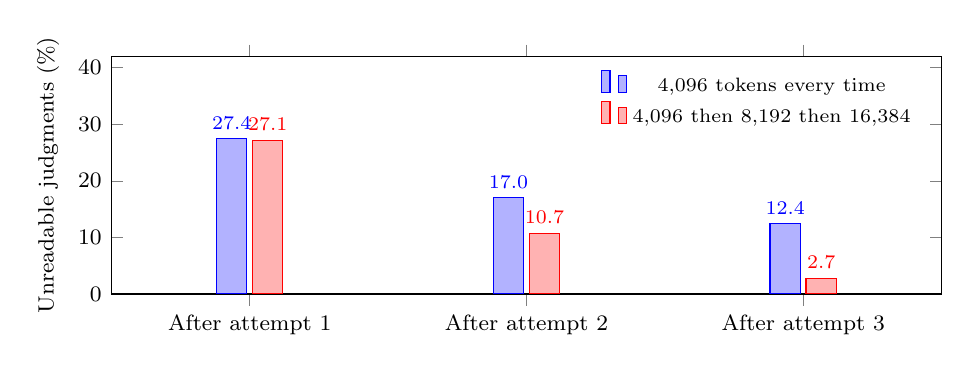
\begin{tikzpicture}
    \begin{axis}[
        ybar,
        width=\columnwidth,
        height=4.6cm,
        bar width=11pt,
        ymin=0, ymax=42,
        ylabel={Unreadable judgments (\%)},
        symbolic x coords={1,2,3},
        xtick=data,
        xticklabels={After attempt 1, After attempt 2, After attempt 3},
        x tick label style={font=\footnotesize},
        y tick label style={font=\footnotesize},
        ylabel style={font=\footnotesize},
        nodes near coords,
        nodes near coords style={font=\scriptsize},
        point meta=explicit symbolic,
        legend style={font=\scriptsize, at={(0.98,0.97)}, anchor=north east, draw=none},
        enlarge x limits=0.25,
      ]
      \addplot coordinates {(1,27.4) [27.4] (2,17.0) [17.0] (3,12.4) [12.4]};
      \addplot coordinates {(1,27.1) [27.1] (2,10.7) [10.7] (3,2.7) [2.7]};
      \legend{{4,096 tokens every time},{4,096 then 8,192 then 16,384}}
    \end{axis}
  \end{tikzpicture}
  \caption{Share of the 9,838 rag26 judgments by gpt-oss-20b that were still
  unreadable after each attempt. One run keeps the reply budget fixed, while the
  other doubles it on each retry. The first attempt gets the same budget in both
  runs. Its result still differs slightly because some answer keys were rebuilt.}
  \label{fig:budget}
\end{figure}

Figure~\ref{fig:budget} shows what the reply budget does. With 4,096 tokens on
every attempt, 12.4\% of the rag26 judgments by gpt-oss-20b were still unreadable
after three attempts. Giving the retries 8,192 and then 16,384 tokens cut this to
2.7\%, or 264 judgments in all. For the second run we also rebuilt the answer keys.
Retries while building a key got the larger budget too. That is why the first
attempt differs slightly between the two runs. The same model had left only
0.75\% of its judgments unreadable on the rag25-gen pilot and 2.9\% on ragtime25.
The problem grew large only on the test data. So retry counts are worth watching
on the test run itself, not just on a pilot. Our second \judge{NuggetRecall} code
submission, \run{grave-node}, carries this fix.

One more trap is not silent, but it is easy to walk into. A TREC qrels file, the
standard file of relevance labels, has four columns separated by whitespace. So does
a leaderboard. TIRA finds the leaderboard by that shape, so a qrels file written
next to it makes the upload fail. For this reason neither of our judges writes a
qrels file. A script also checks every output folder before upload.

\section{Submitted Systems}
\label{sec:submissions}

Table~\ref{tab:submissions} lists what we submitted. A partial leaderboard is
rejected, so every data submission covers every run and every topic of its test
set. A script checked this before each upload.

\begin{table}
  \caption{Our submissions. We produced the data submissions ourselves. The
  organizers ran the code submissions with their own models. A dot marks each test
  set a system covers.}
  \label{tab:submissions}
  \small
  \setlength{\tabcolsep}{4pt}
  \begin{tabular}{@{}lllcc@{}}
    \toprule
    System & Judge & Model & rag26 & ragtime26\\
    \midrule
    \multicolumn{5}{@{}l}{\emph{Data submissions}}\\
    \run{nuggetrecall-best}    & NuggetRecall & Qwen3-30B   & $\bullet$ & $\bullet$\\
    \run{nuggetrecall-rank}    & NuggetRecall & Qwen3-30B   & $\bullet$ & $\bullet$\\
    \run{nuggetrecall-gptoss}  & NuggetRecall & gpt-oss-20b &           & $\bullet$\\
    \run{ensemble-qwen-gptoss} & NuggetRecall & both        & $\bullet$ &          \\
    \run{corroborate-best}     & Corroborate  & none        & $\bullet$ & $\bullet$\\
    \midrule
    \multicolumn{5}{@{}l}{\emph{Code submissions}}\\
    \run{rank-dioptre}         & NuggetRecall & organizers' & $\bullet$ & $\bullet$\\
    \run{grave-node}           & NuggetRecall & organizers' & $\bullet$ & $\bullet$\\
    \run{lead-racer}           & Corroborate  & none        & $\bullet$ & $\bullet$\\
    \bottomrule
  \end{tabular}
\end{table}

\run{nuggetrecall-best} is our main system. Under the scoring in place at the time,
\judge{NuggetRecall} beat \judge{Corroborate} on both pilots that resemble the test
sets. \run{nuggetrecall-rank} adds the within-topic percentile measure
\texttt{NR\_RANK} to the same judgments. We computed it from the submitted
leaderboard instead of judging again, so the run-to-run noise of
Section~\ref{sec:noise} cannot enter. On rag25-gen our computation matches the
judge's own to twelve decimal places.

We added \run{nuggetrecall-gptoss} because gpt-oss-20b was our best judge on
ragtime25. On ragtime26 it left 163 of 5,041 judgments unreadable (3.2\%). It also fell back to a title-only key on 3 of 103 topics. We included the ensemble
\run{ensemble-qwen-gptoss} for its gain in \tauap\ on rag25-gen
(Section~\ref{sec:ensemble}). \run{corroborate-best} is our LLM-free method. It
shares its configuration with \run{lead-racer}, including the 0.50 specificity
floor.

The two \judge{NuggetRecall} code submissions differ in only one way.
\run{grave-node} carries the growing reply budget of Section~\ref{sec:budget},
which doubles the token limit on each retry. \run{rank-dioptre} does not. We
registered \run{grave-node} after we saw what a fixed budget did to gpt-oss-20b on
rag26 (Figure~\ref{fig:budget}). We then asked the organizers to treat it as our
main code submission.

\subsection{Test-set results}

\pending{The organizers have not released test-set scores yet. Add a table here with
Kendall and \tauap\ per truth measure for every system in
Table~\ref{tab:submissions}, including each model the organizers ran our code
submissions with, and compare it with the pilot predictions in
Section~\ref{sec:results}.}

\section{Limitations}

\begin{itemize}
  \item We made every score-based choice on the 2025 pilots, as the rules require.
    They have 28 to 59 systems each, so the 2026 results may differ from what the
    pilots suggest.
  \item The organizers re-scored the pilots after we had made our choices. The
    ensemble for rag26 looks better under the earlier scoring than under the
    current one.
  \item On dragun-repgen our local runs used different topic text from the copy on
    TIRA. We do not know whether the test sets on TIRA match the released files,
    and our data submissions used the released files.
  \item \judge{NuggetRecall} depends on the LLM's own knowledge to write the answer
    key, and on the request being a real information need. It never sees
    citations, so it cannot judge attribution.
  \item \judge{Corroborate} cannot reward a correct fact that no other team stated.
    Consensus is a proxy for importance, not a measure of it, and a correct but rare
    fact gets little weight. We did not run the ablations that would show how much
    the leave-one-team-out weight and per-team voting each change the ranking.
  \item Without truth on the test sets we could check only that our leaderboards
    were complete and that every measure varied across systems. We ran no length
    diagnostics on them. A script may compute such a statistic, but the policy
    treats the result as restricted, and it could have steered choices that must
    come from the pilots.
\end{itemize}

\section{Data Handling and Reproducibility}
\label{sec:disclosure}

Development followed the AutoJudge data policy. On the test sets we read response
content only for the first ten topics of each topics file, in file order, and every
choice we made by score came from the pilots. Every bug but one reproduced on a
pilot or on the synthetic dataset that ships with the starter kit, so we never
needed the policy's scrubbing tool. The exception is the exhausted reply budget of
Section~\ref{sec:failures}. It also occurs on the pilots, at lower rates, but we
noticed it on rag26 and saw it there only as counts: unreadable judgments in our
logs, and requests that vLLM stopped at the length limit. We read no response text
to diagnose it. The answer keys of \judge{NuggetRecall} are built from the topic
alone, so they may be read for any topic. The claim banks of \judge{Corroborate}
are built from responses, and we inspected them only on the pilots.

We also submitted two generation runs to TREC 2026 RAG, so two of the 83 rag26 runs
are probably ours. We made no attempt to identify them, by comparison with our own
submissions or by any other means. Neither judge knows which runs are ours, and
both treat every run alike. \judge{NuggetRecall} judges each response on its own
against a key built from the topic. \judge{Corroborate} drops a team's own vote
from each claim's weight, so a team's runs cannot raise the weight of the claims
they are scored on.

Both judges are available as code submissions on TIRA. The source code, workflows
and tests are at \pending{public repository URL}. \judge{NuggetRecall} reproduces
from its prompt cache with the endpoint switched off. \judge{Corroborate} makes no
network calls, and on the same inputs and hardware it produces byte-identical
output.

\section{Summary}

We built two judges for TREC 2026 AutoJudge that fail in different places.
\judge{NuggetRecall} writes an answer key from the question and does best on nugget
coverage. \judge{Corroborate} trusts what many teams agree on, does best on F1 for
long reports and fails on short answers. The largest effect we measured was the
choice of judge model. The most useful lessons, though, concern failure. An LLM
judge can lose most of its judgments without an error and still produce a
leaderboard that looks plausible. A check that measures vary across systems, retry
counts watched on the real data, and a liveness check beside every reproducibility
check caught most such failures. An audit aimed at exactly this kind of failure
caught the rest.


\begin{acks}
We thank the AutoJudge organizers and the TIRA team for running our code
submissions with their own models and for answering our questions quickly.
\pending{Funding and compute acknowledgments.}
\end{acks}

\bibliographystyle{ACM-Reference-Format}
\bibliography{references}

\appendix
\section{Prompts}
\label{app:prompts}

Both prompts of \judge{NuggetRecall}, verbatim. Text in braces is filled in at run
time. Each is sent as a single user message at temperature 0.

\paragraph{Answer key.} Called once per topic, with \texttt{min\_n}=8 and
\texttt{max\_n}=20.
\begin{lstlisting}
You are building the answer key for evaluating responses to an information request.

REQUEST:
{request}

List the key facts that a complete, high-quality response to this request should contain. Each item must be:
- one self-contained factual statement, a single idea per line
- specific enough that you could check whether a response states it
- relevant to what the request actually asks for

Mark an item VITAL if a response that omits it is clearly incomplete, or OKAY if it is useful supporting detail.

Give between {min_n} and {max_n} items, most important first. Output only the list, one item per line, in exactly this format and nothing else:
1. [VITAL] <fact>
2. [OKAY] <fact>
\end{lstlisting}

\paragraph{Judging.} Called once per response. The facts are numbered from 1, one per
line.
\begin{lstlisting}
You are checking which facts a response covers. Judge only what the response says. Never use outside knowledge.

REQUEST:
{request}

RESPONSE TO JUDGE:
{answer}

FACTS TO CHECK (one per line, numbered):
{facts}

For every numbered fact, decide whether the RESPONSE conveys it:
  support  - the response clearly states this fact
  partial  - the response states part of it, gestures at it, or hedges it
  no       - the response does not convey it

Judge meaning, not wording: the same fact stated in different words is support. A fact the response merely names as a topic, without asserting it, is partial.

Output exactly one line per fact, in order, and nothing else:
1: support
2: no
3: partial

Output {count} lines, numbered 1 to {count}.
\end{lstlisting}

\paragraph{Retry suffixes.} The first attempt sends the prompt as is. The second
attempt appends the first line below and the third attempt the second, each after
a blank line. Both prompts use the same suffixes.
\begin{lstlisting}
Reminder: follow the output format exactly, with no other text.
Important: output only the numbered lines, exactly as specified, nothing else.
\end{lstlisting}


\end{document}
